\documentclass{article}

\usepackage{amsfonts, amsmath, amsthm, graphicx, color}
\usepackage[boxed,linesnumbered]{algorithm2e}
\DontPrintSemicolon
\SetArgSty{}

\title{Lecture 8 Scratchwork}
\author{COT 4400, Fall 2015}

\newcommand{\Z}{\mathbb{Z}}
\newcommand{\Q}{\mathbb{Q}}
\newcommand{\R}{\mathbb{R}}
\newcommand{\N}{\mathbb{N}}
\newcommand{\T}{\textbf{true}}
\newcommand{\F}{\textbf{false}}
\newcommand{\liff}{\leftrightarrow}

\definecolor{dkred}{rgb}{0.5,0,0}
\newcommand{\ans}[1]{}
%\newcommand{\ans}[1]{\color{dkred}\textbf{Answer:} #1\color{black}}

\newtheorem{counterexample}{Counterexample}

\begin{document}
\maketitle

%%%%%%%%%%%%%%%%%%%%%%%%%%%%%%%%%%%%%%%%%%%%%%
% Correctness and analysis                   %
%%%%%%%%%%%%%%%%%%%%%%%%%%%%%%%%%%%%%%%%%%%%%%


\begin{algorithm}
\KwIn{$data$:  an array of integers to sort}
\KwIn{$n$:     the number of values in data}
\KwOut{permutation of data such that $data[1] \leq \ldots \leq data[n]$}
\TitleOfAlgo{BubbleSort}
\Repeat {the \KwSty{for} loop makes no swaps} %line 1 (until condition line 5)
{
  \For{$i = 1$ to $n-1$} %line 2
  {
    \uIf {$data[i] > data[i+1]$} %line 3
    {
      Swap $data[i]$ and $data[i+1]$\; %line 4
    }
  }
} %until (line 5)
\Return{$data$}\; %line 6
\end{algorithm}

\begin{enumerate}
\item Prove that Bubble Sort is correct.











\newpage
\item Prove a tight upper bound on the worst-case complexity of Bubble Sort.

\textit{Hint:}
After iteration $k$ of the outer loop in Bubble Sort (line 1),
the last $k$ values will be the largest $k$ values in the array,
in sorted order.

\textbf{Solution:}

The inner loop iterates $n - 1 = O(n)$ times, and each iteration costs $O(1)$, for a total time of $O(n)O(1) = O(n)$.  

Claim:  the outer loop iterates $O(n)$ times in the worst case.

Consider an array sorted in decreasing order.  By the end of the first iteration, the largest value (data[1]) will be swapped to data[n], and every other value will be shifted to the left.  In the second iteration, data[1] will get swapped to data[n-1] and all values in between will be shifted one to the left.  This will continue until the $(n-1)^\textrm{st}$ iteration, when data[1] will be swapped into data[2].  On the next iteration, all of the values data[1], \ldots, data[n] will be in sorted order, so no swaps will be made, so the outer loop will terminate.  Total iterations:  $n$ iterations.

Therefore, the outer loop may iterate $O(n)$ times in the worst case, for a total time of $O(n^2)$.  This time dominates the $O(1)$ cost for the return statement, so the entire algorithm will be $O(n^2)$.

%%%%%%%%%%%%%%%%%%%%%%%%%%%%%%%%%%%%%%%%%%%%%%
% Big-Oh                                     %
%%%%%%%%%%%%%%%%%%%%%%%%%%%%%%%%%%%%%%%%%%%%%%

\newpage
% Problem 1
\item Prove the multiplicative envelopment property of Big-Omega:

$j(n)k(n) = \Omega(f(n)g(n))$, 
where $j(n) = \Omega(f(n))$ and $k(n) = \Omega(g(n))$
\\

Assumptions:  $j(n) = \Omega(f(n))$ and $k(n) = \Omega(g(n))$

Show:  $j(n)k(n) = \Omega(f(n)g(n))$

\begin{proof}
Since $j(n) = \Omega(f(n))$, there exists $c_1, n_1$ such that                              $j(n) \geq c_1f(n)$ for all $n \geq n_1$.  
Similarly, $k(n) \geq c_2g(n)$ for all $n \geq n_2$, for some positive constants $c_2$ and $n_2$.
Since $j(n), k(n), f(n), g(n), c_1$, and $c_2$ are positive, we can multiply both sides of the inequalities, and we get
$j(n)k(n) \geq c_1c_2f(n)g(n)$ for all $n \geq n_3$. where $n_3 = \max\{n_1, n_2\}$.  Let $c_3 = c_1c_2$.  
Therefore, there exist positive constants $c_3$ and $n_3$ such that                                     $j(n)k(n) \geq c_3f(n)g(n)$ for all $n \geq n_3$,
so $j(n)k(n) = \Omega(f(n)g(n))$ by the definition of Big-Omega.
\end{proof}



\newpage
% Problem 2
\item Prove that if $g(n) \neq O(1)$, $f(n)g(n) \neq O(f(n))$.



%%%%%%%%%%%%%%%%%%%%%%%%%%%%%%%%%%%%%%%%%%%%%%
% Algorithm design                           %
%%%%%%%%%%%%%%%%%%%%%%%%%%%%%%%%%%%%%%%%%%%%%%

\newpage
\item Design a greedy algorithm that finds a graph coloring.

\textbf{Problem:}  Graph coloring
\begin{itemize}
\item \textbf{Input:}  a graph network $G$ and a coloring number $n$
\item \textbf{Output:}  an assignment of colors $(1..n)$ to the nodes of $G$ such that no nodes connected by an edge are the same color, or ``no such coloring'' if none exists
\item \textbf{Example:}  $n = 3$

\begin{tabular}{rl}
$G$: & 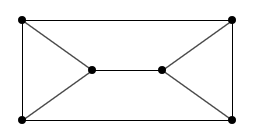
\includegraphics[width=2in]{coloring-example.png}\\
\textbf{Possible solution:} & 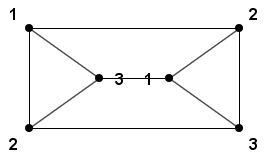
\includegraphics[width=2in]{coloring-soln.png}
\end{tabular}
\end{itemize}

\textit{Hint}:  $N(v)$ is the set of neighbors of $v$; i.e., the vertices joined to $v$ by an edge


%%%%%%%%%%%%%%%%%%%%%%%%%%%%%%%%%%%%%%%%%%%%%%
% Recurrences                                %
%%%%%%%%%%%%%%%%%%%%%%%%%%%%%%%%%%%%%%%%%%%%%%

\newpage
\item Identify the worst-case complexity of the PolyEval algorithm (below):

\begin{algorithm}
\KwIn{$d$:  the degree of the polynomial to evaluate}
\KwIn{coeff:  the coefficients of the polynomial (largest to smallest)}
\KwOut{the value of $f(x)$}
\TitleOfAlgo{PolyEval}
\eIf{$d = 0$}
{
  \Return{coeff$[1]$}\;
}
{
  Let $temp = $PolyEval$(d-1, $coeff$[1..d-1], x)$\;
  \Return{$x * temp + $coeff$[d]$}\;
}
\end{algorithm}

Let $T(d)$ represent the number of instructions required to evaluate a polynomial of degree $d$.

$T(0) = O(1)$

If $d > 0$ and we make a copy of the coeff[1..d-1] array, the copy will take $O(n)$ time, the recursive call will take $T(d-1)$ time, and everything else will take constant time, for a total of $T(d) = T(d-1) + O(n)$.

Characteristic equation:  $c(x) = x - 1$.  The zero of this equation is $r = 1$.
The general form of our solution will be $T(n) = d_1(1^n) + O(n^mf(n)) = O(1^n) + O(n^1)O(n) = O(1) + O(n^2) = O(n^2)$.

If we are using pointers, this is reduced to $T(d) = T(d-1) + O(1)$.
Characteristic equation:  $c(x) = x - 1$.  The zero of this equation is $r = 1$.
The general form of our solution will be $T(n) = d_1(1^n) + O(n^mf(n)) = O(1^n) + O(n^1)O(1) = O(1) + O(n) = O(n)$.

\end{enumerate}
\end{document}
